\documentclass{beamer}
\usepackage{
    graphicx, float, caption,
    amsmath,
    textpos, blindtext, scrextend,
    apacite
}
\usepackage[font=small, labelfont=bf]{subcaption}

%% MARK: Beamer Setup
\usetheme{Darmstadt}
% Remove the useless and unsightly black bar at the top of the slides
\setbeamertemplate{headline}{}
% Remove the navigation thing at the bottom of the slides.
\setbeamertemplate{navigation symbols}{}
% Colors for Auburn University from their marketing materials
% http://www.ocm.auburn.edu/graphicservices/colors.html
\definecolor{auburn_orange}{RGB}{232, 119, 34}
\definecolor{auburn_blue}{RGB}{12, 35, 64}
% Set the color of the slide headers to auburn blue
\setbeamercolor{structure}{fg=auburn_blue}

%% MARK: Frontmatter
\title{Playing Super Mario Bros. with Deep-$Q$ Learning}
\author{Christian Kauten, Chaowei Zhang}
\institute{Auburn University}
\date{April 23, 2018}

%% MARK: Slides
\begin{document}
% title slide
\frame{\titlepage}

\begin{frame}{Problem}
\begin{minipage}{\textwidth}
%
\begin{minipage}{0.5\textwidth}
\begin{itemize}
    \item{Super Mario Bros.}
    \item{Atari 2600}
    \begin{itemize}
    \item{Breakout, Enduro, Pong, Seaquest, Space Invaders}
    \end{itemize}
\end{itemize}
\end{minipage}
\hfill
\begin{minipage}[t]{0.5\textwidth}
\centering
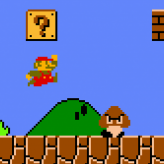
\includegraphics[width=0.85\textwidth]{img/smb} \\
$\Downarrow$ \\
$f : \mathcal{S} \to \mathcal{A}$ \\
$\Downarrow$ \\
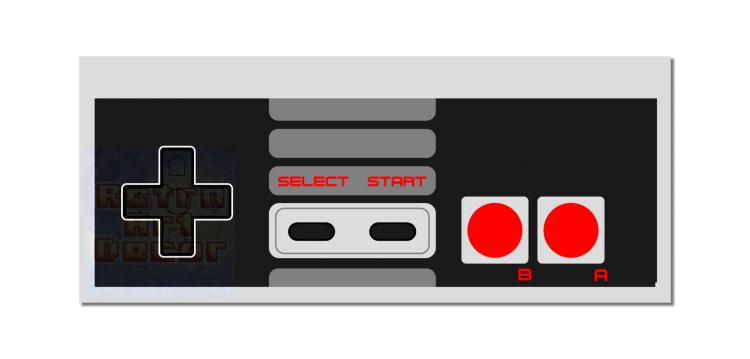
\includegraphics[width=0.85\textwidth]{img/nes}
\end{minipage}
%
\end{minipage}
\end{frame}

\begin{frame}{Dataset}
TODO
\end{frame}

\begin{frame}{Methods}
TODO
\end{frame}

\begin{frame}{Results}
TODO
\end{frame}

\begin{frame}{Demo}
TODO
\end{frame}

\begin{frame}{Conclusions}
TODO
\end{frame}

\begin{frame}{Q\&A}
TODO
\end{frame}

\end{document}
